% !TeX root = ../main.tex
% Add the above to each chapter to make compiling the PDF easier in some editors.

\chapter{Performance Analysis}\label{chapter:performance_analysis}

In this chapter we will test our backends performance and compare it to other backends.
First we will explain the setup used for testing.
We then go on to test and analyse the throughput of our backend with LAIKs ping pong example application.

\section{Setup}

To test our backend the Leibnitz Rechenzetrum (LRZ) provided us with access to its testing environment BEAST.
We tested our setup on the ice cluster of the LRZ BEAST. 
This cluster consists of two Intel Xeon Platinum 8360Y CPUs running on 2.40GHz.
Every CPU has 2 sockets with 36 cores each.

We tested our secondary backend version integrated into an MPI backend against two versions of the LAIK MPI backend. 
Th first one used a shared memory fabric and the second one a tcp fabric.
LAIK was compiled with gcc 11.2.0 and intel mpi version 2021.4.0.

The MPI backend was run with the environment variable \code{I\_MPI\_ASYNC\_PROGRESS} set to 1.
This enables asynchronous progress threads which achieve better communication/computation overlapping\cite{intel-mpi}. 
When using the shared memory fabric we set \code{I\_MPI\_SHM} to \code{icx} to choose the shared memory transport solution for Intel Xeon processors with Ice Lake microarchitecture \cite{intel-mpi}.
We also set the \code{I\_MPI\_OFI\_PROVIDER} to shm to choose shared memory for transportation.
The \code{I\_MPI\_SHM\_CMA\_THRESHOLD} variable was set to 2000000000 to ensure that shared memory was used despite of the large sizes involved.
When we used the tcp fabric we set \code{I\_MPI\_OFI\_PROVIDER} to tcp to use tcp for transportation.
We also set \code{FI\_LOG\_LEVEL} to debug to be able to confirm through the debug information, that the correct fabric was used\cite{intel-mpi}.

\section{Ping Pong}

The ping pong example is one of the examples provided in the LAIK library.
It moves an array of doubles repeatedly between processes.
We can set the arrays size as well as the repetitions over command line arguments.
Ping pong performs the data migrations between pairs of processes with even and odd rank ((1,2), (2,3), ...).

We used the Ping Pong example to measure and compare the throughput of the tested backends.
The throughput in GB/s is a good indicator of a backends performance as it measures how fast a backend can transport data between processes.
We tested the ping pong example with an array size of 100 million doubles and 10 iterations.

\subsubsection{Throughput}
\begin{figure}[h]
	\centering
	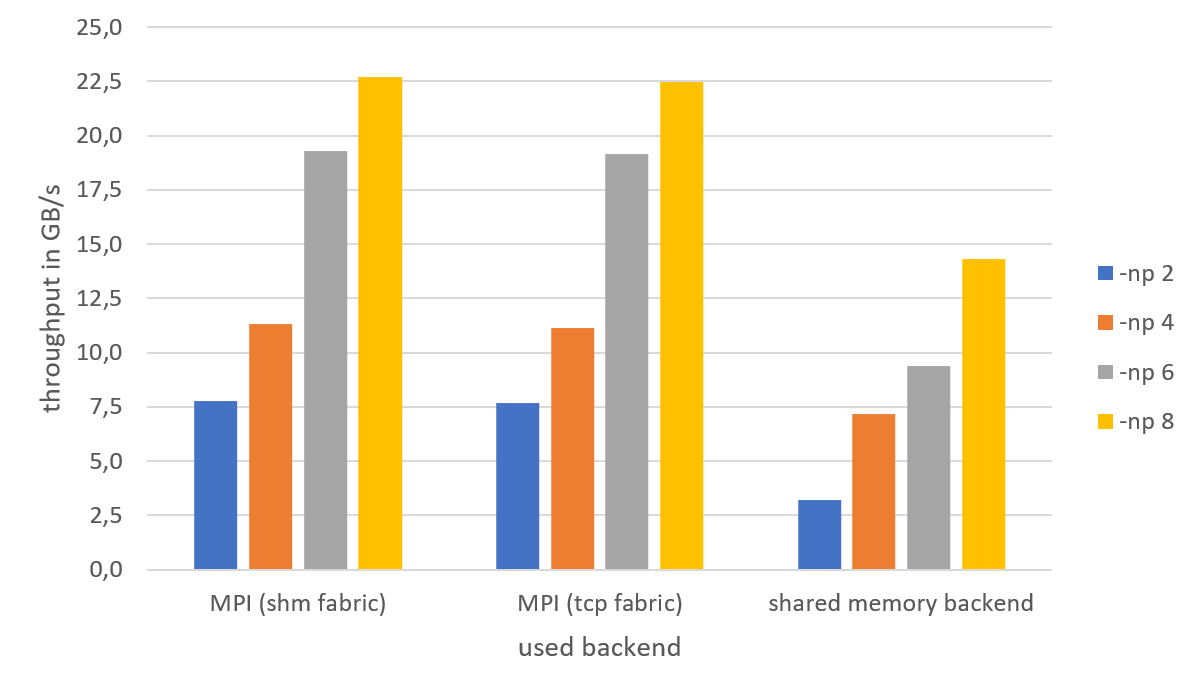
\includegraphics[width=0.75\columnwidth]{figures/throughput.png}
	\caption{Throughput of the different backends with different group sizes.}
	\label{fig:throughput}
\end{figure}

In our first test we measured the throughput of the backends at different process numbers. 
As we can see in \autoref{fig:throughput}, the backends throughput increases with the number of processes.
This was to be expected as more processes are able to send more data.
The two versions of the MPI backend nearly achieve similar performance regardless of the used fabric.
Only our shared memory backend is lacking in performance which is unexpected.
Through profiling we could find out, that the linked \code{memcpy()} call used in the data migration was slow.
The call alone took longer than a \code{MPI\_Send()} call for an array of equal size.
This is due to a slow implementation of \code{memcpy()} being linked to our backend during compilation.
The performance of the backend would have likely been better if a more performant \code{memcpy()} call was linked to it.
Unfortunately, we could not complete this within the scope of our work.

\subsubsection{Influence of the Deployment on Performance}

We also tested how the throughput of our backend changes depending on the deployment of our processes.
We deployed the ping pong example with two processes on different processors to see the influence the deployment had on the performance.
The processes were pinned to the processors by using the environment variable \code{I\_MPI\_PIN\_PROCESSOR\_LIST}.

\begin{figure}[h]
	\centering
	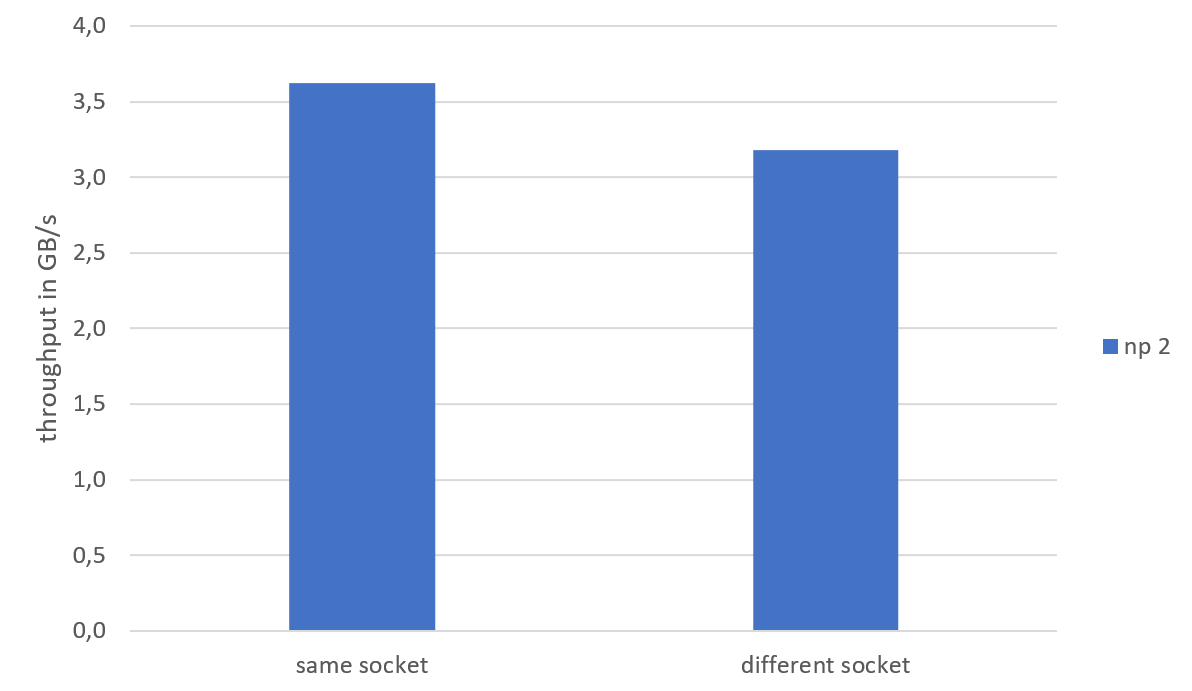
\includegraphics[width=0.70\columnwidth]{figures/socket.png}
	\caption{Throughput of ping pong with two processes on the same and on different sockets}
	\label{fig:socket}
\end{figure}

First we tested how the throughput differs between two processes deployed on the same socket and two processes being deployed on different sockets.
One would expect the 2 processes on the same socket to be faster.
Our tests confirmed that two processes on the same socket achieve around 0.5GB/s more throughput than the processes on different sockets (see \autoref{fig:socket}). 

\begin{figure}[h]
	\centering
	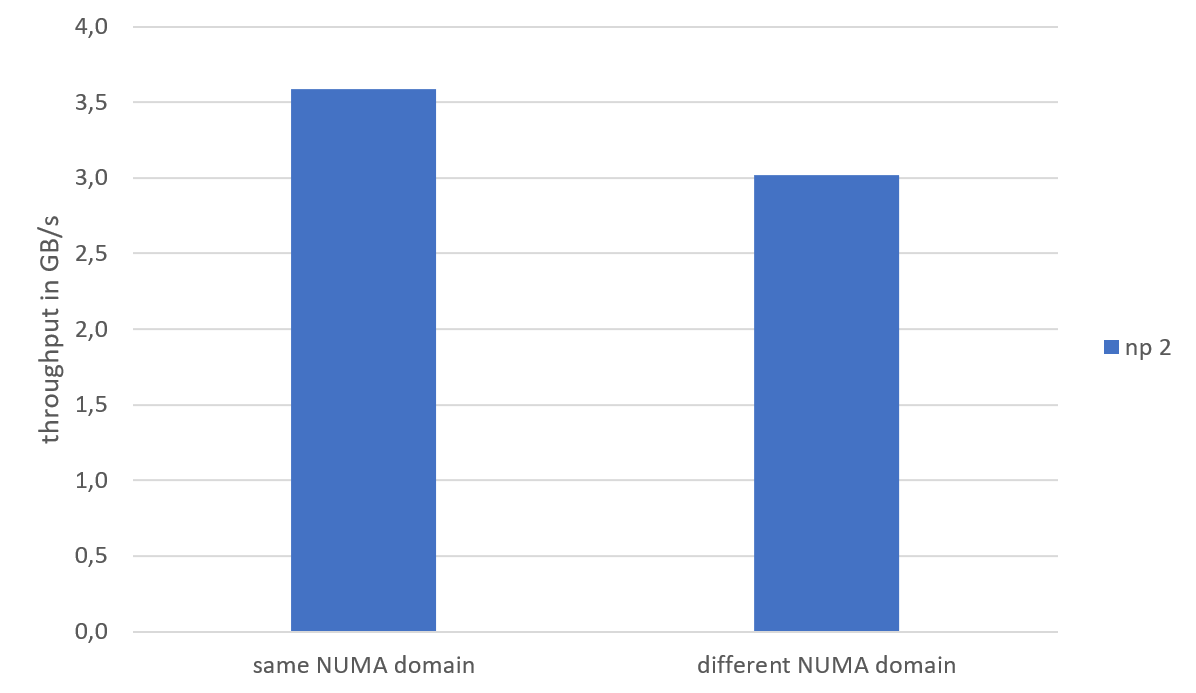
\includegraphics[width=0.70\columnwidth]{figures/numa.png}
	\caption{Throughput of ping pong with two processes in the same and in different NUMA domains}
	\label{fig:numa}
\end{figure}

The influence of NUMA domains on the throughput was also examined.
Processes in the same NUMA domain are expected to achieve a higher throughput.
As we can see in \autoref{fig:numa} the processes in the same NUMA domain achieved a higher throughput than those in different NUMA domains.

\subsubsection{Comparison between 2 and 1 Copy Data Transport}

Finally, we compared the 2 copy data transport against the 1 copy data transport to see how big the performance difference between the 2 versions is.
It is expected, that the 1 copy version achieves a higher throughput since it uses one \code{memcpy()} operation less than the 2 copy version.
\autoref{fig:2vs1} shows that the 1 copy versions throughput is more than twice as high as the throughput of the 2 copy version.
Besides the additional \code{memcpy()} call, the 2 copy version also has to create and destroy a shared memory segment for each data migration which adds aditional overhead.
It is therefore no surprise that the 1 copy versions performance is far better. 

\begin{figure}[h]
	\centering
	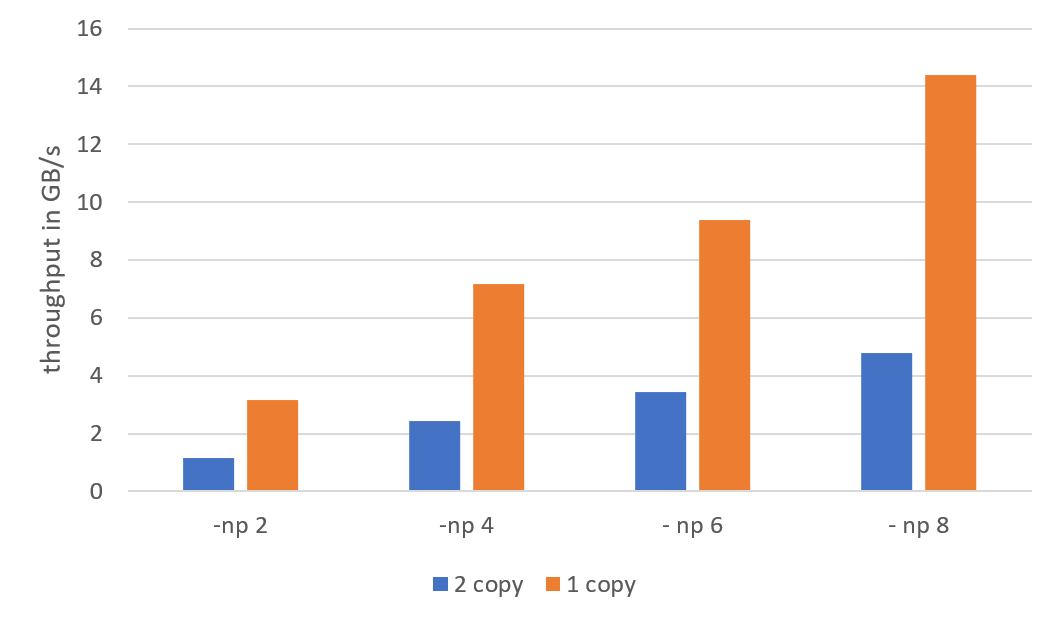
\includegraphics[width=0.70\columnwidth]{figures/2vs1.png}
	\caption{Comparison between the throughput of the 2 copy and the 1 copy data transport}
	\label{fig:2vs1}
\end{figure}